\section{SECCIÓN 1. PROPÓSITO}

El presente Plan de Aseguramiento de la Calidad está orientado a una Galería de Imágenes Segura desarrollada con Spring Boot, React y PostgreSQL, cuya principal característica es la detección de contenido oculto mediante técnicas de análisis de esteganografía. Con este documento se establece el alcance, la estrategia de las pruebas, los criterios de aceptación, las herramientas a utilizarse y la gestión de riesgos asociados al sistema, con el propósito de garantizar su correcto funcionamiento, fortalecer su nivel de seguridad y asegurar una experiencia confiable para los usuarios finales a través de un proceso estructurado de validación y mejora continua.

\subsection{1.1 ALCANCE}
El sistema bajo prueba (SUT) es una Galería de Imágenes Segura (backend Spring Boot 4.0.6 / Java 21 + frontend React 18 + Vite, persistencia en PostgreSQL). Sus principales módulos a probar son: Gestión de autenticación de usuarios, carga y almacenamiento de imágenes, organización en álbumes, detección de esteganografía basada en análisis de anomalías LSB (bits menos significativos) y metadatos EXIF, cuarentena de archivos sospechosos, y un panel de supervisor para auditoría.

Se realizará una identificación de puntos clave del sistema, herramientas y definición de mediciones para la correcta evaluación de las funcionalidades. Finalmente, se presentará un reporte de los hallazgos y posibles mejoras dentro del sistema.

\subsection{1.2 VISIÓN GENERAL DEL SISTEMA}
El sistema [Nombre del Sistema] \textit{completar la oración proporcionando una descripción del sistema y el uso previsto}. El sistema incluye [número de subsistemas, ej., 4] subsistema(s) dentro del sistema. La Figura 1-1 identifica los CI dentro de cada subsistema y destaca aquellos a los que se aplica este Plan SQA.

\begin{table}[H]
\centering
\caption{Actividades del Ciclo de Vida del Software}
\label{tab:lifecycle}
\begin{tabular}{|c|}
\hline
\textbf{ACTIVIDAD DEL CICLO DE VIDA DEL SOFTWARE} \\
\hline
Planificación y Supervisión del Proyecto \\
\hline
Entorno de Desarrollo de Software \\
\hline
Análisis de Requisitos del Sistema \\
\hline
Diseño del Sistema \\
\hline
Análisis de Requisitos del Software \\
\hline
Diseño del Software \\
\hline
Implementación del Software y Pruebas Unitarias \\
\hline
Pruebas de Integración de Unidades \\
\hline
Pruebas de Calificación de CI \\
\hline
Pruebas de Integración CI/CIHW y del Sistema \\
\hline
Pruebas de Calificación del Sistema \\
\hline
Preparación para el Uso del Software \\
\hline
Preparación para la Transición del Software \\
\hline
Mantenimiento del Ciclo de Vida \\
\hline
\end{tabular}
\end{table}

\begin{table}[H]
\centering
\caption{Nomenclatura/Identificación de CI}
\label{tab:ci}
\begin{tabular}{|p{4cm}|p{3cm}|p{3cm}|}
\hline
\textbf{NOMENCLATURA} & \textbf{ACRÓNIMO} & \textbf{NÚMERO DE CI} \\
\hline
[Doc 1] & [Acrónimo] & [ID del CI] \\
\hline
\end{tabular}
\end{table}

\subsection{1.3 VISTA GENERAL DEL DOCUMENTO}
Este documento identifica las organizaciones y procedimientos que se utilizarán para realizar las actividades relacionadas con el programa SQA del proyecto, según lo especificado en el estándar IEEE Std 730-1998, \textit{IEEE Standard for Software Quality Assurance Plans}, referencia (c), y IEEE Std 730.1-1995, \textit{IEEE Guide for SQA Planning}, referencia (d).

La Sección 1 identifica el sistema al que se aplica este Plan SQA; proporciona una visión general del sistema y sus funciones de software; resume el propósito y el contenido del Plan SQA; describe la relación del Plan SQA con otros planes de gestión y enumera todos los documentos referenciados en este Plan SQA.

La Sección 2 describe cada elemento principal de la organización que influye en la calidad del software.

\begin{figure}[H]
\centering
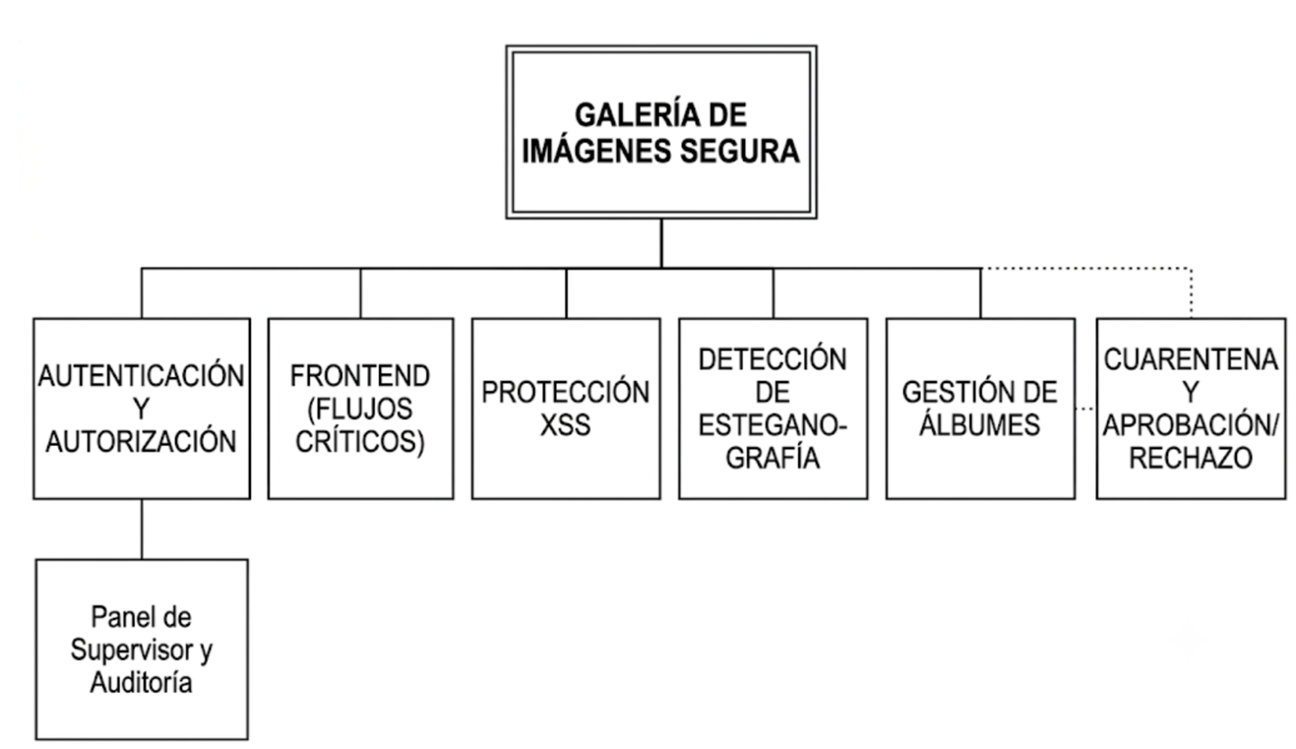
\includegraphics[width=0.8\textwidth]{images/imagen1.png}
\caption{Software de [Título del Sistema]}
\label{fig:system}
\end{figure}

La Sección 3 describe las diversas tareas de SQA.
La Sección 4 enumera los documentos base producidos y mantenidos por el proyecto.
La Sección 5 identifica los estándares, prácticas y convenciones.
La Sección 6 describe la participación de SQA en las pruebas.
La Sección 7 describe el reporte de problemas y la acción correctiva.
La Sección 8 describe las herramientas, técnicas y metodologías de SQA.
La Sección 9 describe la herramienta de gestión de configuración utilizada para el control del código.
La Sección 10 describe la evaluación de SQA del control de medios.
La Sección 11 describe el control del software de proveedores.
La Sección 12 describe los procedimientos de SQA para la recopilación, mantenimiento y retención de registros.
La Sección 13 describe los requisitos de capacitación de SQA.
La Sección 14 describe la revisión de SQA del proceso de Gestión de Riesgos.
El Apéndice A proporciona una lista de acrónimos.
El Apéndice B proporciona listas de verificación que se utilizarán o adaptarán para verificar el cumplimiento de las mejores prácticas generales de ingeniería de software.

\subsection{1.6 DOCUMENTOS DE REFERENCIA}
\begin{enumerate}
    \item SSC San Diego Software Quality Assurance Policy, Version 1.1, October 1997.
    \item IEEE/EIA Standard 12207 Series - Standard for Information Technology – Software life cycle processes, March 1998.
    \item IEEE-Std-730-1998, IEEE Standard for Software Quality Assurance Plans, June 1998.
    \item IEEE-Std-730.1-1995, IEEE Guide for Software Quality Assurance Planning, December 1995.
    \item Multimedia gallery steganography
detection safe Software Development Plan, [Identificación del Documento], [Fecha del Documento].
    \item Multimedia gallery steganography
detection safe Software Configuration Management Plan, [Identificación del Documento], [Fecha del Documento].
    \item Software Engineering Process Policy, SPAWARSYSCEN SAN DIEGO INST 5234.1, July 2000.
    \item Multimedia gallery steganography detection safe Program Plan, [Identificación del Documento], [Fecha del Documento].
    \item Software Quality Assurance Process, PR-SQA-02.
    \item Software Quality Assurance Plan Template, TM-SQA-01.
    \item A Description of the Space and Naval Warfare System Center San Diego Software Process Assets, PR-OPD-03.
    \item MIL-STD-1521, Technical Reviews and Audits for Systems, Equipments, and Computer Software.
    \item MIL-STD-973, Configuration Management. NOTA: Esta norma ha sido reemplazada por EIA-649, el Estándar de Consenso para la Gestión de Configuración, pero las disposiciones de MIL-STD-973 se consideran útiles como guía para desarrollar actividades de Gestión de Configuración de Software.
    \item Peer Review Process, PR-PR-02.
    \item Military Standard (MIL-STD)-498, Software Development and Documentation, Data Item Descriptions (DIDs). NOTA: Aunque MIL-STD-498 ha sido reemplazado por IEEE Std 12207, los DIDs para MIL-STD-498 todavía se consideran aplicables para el apoyo al desarrollo de procedimientos de ingeniería de software y documentación de soporte.
    \item IEEE Std 1045-1992, IEEE Standard for Software Productivity Metrics, September 1992.
    \item IEEE Std 1061-1992, IEEE Standard for a Software Quality Metrics Methodology, December 1992.
    \item IEEE Std 982.1-1988, IEEE Standard Dictionary of Measures to Produce Reliable Software, June 1988.
    \item Std 982.2-1988, IEEE Guide for the Use of IEEE Standard Dictionary of Measures to Produce Reliable Software, September 1988.
\end{enumerate}
